\chapter{Аналитическая часть}

\section{Методы визуализации мышц}

Как уже было сказано во введении, все методы визуализации мышц можно разделить на 3 группы:
\begin{itemize}
    \item геометрические;
    \item физические;
    \item методы, основанные на данных.
\end{itemize}

\subsection{Геометрические методы}

Геометрические методы описывают мышцу как поверхность, задаваемую математической функцией или множеством математических функций. Данные методы визуализации мышц использовались в ранних системах, потому что они менее трудоёмкие в сравнении с физическими методами, а также более точны в следствие того, что модель точно задается и описывается функцией без аппроксимации и интерполяции\cite{cgv}. Чаще всего такие методы используются для визуализации сокращения мышц, которые могут использоваться как основа для визуализации деформации кожи и анимации лица. Данные методы позволяют моделировать также и веретенообразные мышцы, используя и комбинируя функции фигур вращения. Учитывая факт ограниченности данных методов из-за использования математических функций в своей основе, а также тот факт, что сокращение мышц определяется возможными сокращениями скелета, данные методы зачастую не позволяют достичь достаточной степени реализма с точки зрения физиологии и биомеханики \cite{bio}.

Наиболее распространённые геометрические методы:
\begin{itemize}
    \item FFD (Free Form Deformation)\cite{ffd};
    \item методы, использующие параметрические и полигональные поверхности\cite{pps};
    \item методы, использующие поверхности, заданные неявными функциями\cite{is1}\cite{is2}.
\end{itemize}

\subsection{Физические методы}

В то время, как геометрический подход к решению задачи визуализации мышц доказал свою применимость в статических графических системах, лежащий в его основе подход описания моделей через математические функции не позволяет работать с динамическими системами, то есть системами, положение которых меняется со временем по законам физики\cite{cgv}. Исследователи подошли к решению проблемы построения динамеческой системы с точки зрения физики.

Физические методы решения задачи визуализации мышц нередко используются совместно с геометрическими, однако основная идея заключается в том, что в них весь объект делится на части и учитывается взаимодействие этих частей между собой в каждый момент времени.


Наиболее распространённые физические методы:
\begin{itemize}
    \item MSS (Mass-Spring System)\cite{mss};
    \item метод конечных элементов (FEM)\cite{fem1}\cite{fem2};
    \item метод конечных объемов (FVM)\cite{fvm1}\cite{fvm2}.
\end{itemize}

\label{phys}
Примером модели мышц на основе физических методов может послужить VIPER\cite{viper} (англ. Volume Invariant Position-based Elastic Rods) - версия модели позиционных эластичных стержней\cite{per} (англ. Position-based Elastic Rods), сохраняющая объем, представленная на конференции SIGGRAPH 2019 \cite{sgr}. С помощью данных моделей мышца представляется в виде набора стержней, состоящих из узлов, имеющих в случае обычной модели 2 параметра для каждого узла: позиция и степень скручивания, а в случае модели, сохраняющей объем - 3 параметра: позиция, степень скручивания и масштаб. Данные модели используются для представления динамической системы. 

\subsection{Методы, основанные на данных}

Эти методы используют данные, которые собираются с поверхности интересующего объекта с помощью системы захвата движения, которая считывает данные с исследуемого объекта при помощи так называемых маркеров. Подобные методы новее методов, перечисленных выше, и нередко позволяют достичь более реальных результатов для определённого объекта, нежели их конкуренты. Однако данный подход решает более частную задачу, что сокращает область его применимости\cite{dda}.

\section{Существующие программные обеспечения}

На рисунках \ref{img:viper_muscle} и \ref{img:viper_muscle2} показано, как выглядят мышцы при использовании модели на основе VIPER, физического метода, описанного в \ref{phys}.

\img{100mm}{viper_muscle}{Мышцы на основе VIPER, прозрачные стержни.}
\img{100mm}{viper_muscle2}{Мышцы на основе VIPER, вид с сеткой.}

Ещё одним популярным продуктом в сфере визуализации мышц является X-Muscle System\cite{xms} - расширение для программы Blender\cite{blender}, которое позволяет создавать мышцы в интерактивном режиме. В данном случае мышца состоит из так называемых \textit{канонических костей}, которые имеют 3 параметра: позиция, направление и ориентация. На рисунках \ref{img:xmuscle} и \ref{img:xmuscle2} показаны примеры мышц, на основе модели X-Muscle System.

\img{75mm}{xmuscle}{Мышцы X-Muscle System. Проектирование.}
\img{75mm}{xmuscle2}{Мышцы X-Muscle System с текстурами.}

\section{Модели мышцы и каркаса}

\subsection{Модель мышцы}

Бицепс является веретенообразной мышцой, что позволяет в полной мере использовать геометрические методы. К тому же программное обеспечение, получаемое в результате данной работы предусматривает статическую систему, что позволяет использовать все преимущства геометрических методов и не иметь проблем их с недостатками.

Ввиду сложности прямого описания поверхности мышцы некоторым уравнением, а также сложности конфигурирования мышцы через параметризованные функции, модель мышцы в данной работе будет представляться с помощью группы усечённых конусов, полученной путем вращения группы отрезков, находящихся между узлами модели. Очевидно, что при такой модели радиусы основания конуса описываются значениями радиусов в точках начала и конца отрезка, которые далее будут называться \textit{радиусом узла}. Такая модель позволяет аппроксимировать функции любого вида с произвольной точностью, а также задавать параметр в каждой точке получающейся табличной функции. Модель с 4 узлами представлена на рисунке \ref{cone}, получена данная модель путем вращения группы отрезков, представленных на рисунке \ref{cone_plane} (отрезки: $r_1r_2$, $r_2r_3$, $r_3r_4$). Чем большая точность требуется, тем большее количество узлов потребуется для аппроксимации мышцы.

\begin{figure}[!ht]
    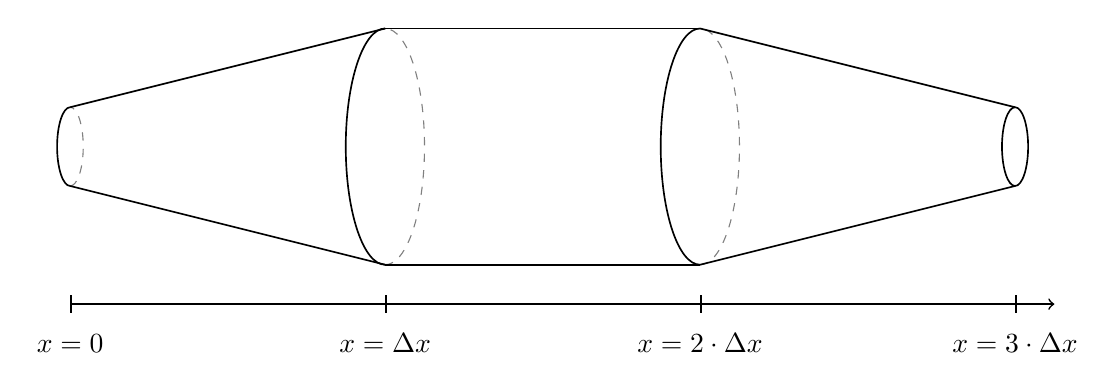
\begin{tikzpicture}
        \draw[dashed,color=gray] (0,1) arc (-90:90:0.166 and 0.5);
        \draw[semithick] (0,1) arc (270:90:0.166 and 0.5);

        \draw[semithick] (4,0) -- (0,1);% bottom line
        \draw[semithick] (4,3) -- (0,2);% top line

        \draw[dashed,color=gray] (4,0) arc (-90:90:0.5 and 1.5);% right half of the left ellipse
        \draw[semithick] (4,0) arc (270:90:0.5 and 1.5);% left half of the left ellipse

        \draw[semithick] (4,0) -- (8,0);% bottom line
        \draw[semithick] (4,3) -- (8,3);% top line

        \draw[dashed,color=gray] (8,0) arc (-90:90:0.5 and 1.5);% right half of the left ellipse
        \draw[semithick] (8,0) arc (270:90:0.5 and 1.5);% left half of the left ellipse

        \draw[semithick] (8,0) -- (12,1);% bottom line
        \draw[semithick] (8,3) -- (12,2);% top line

        \draw[semithick] (12,1.5) ellipse (0.166 and 0.5);% right ellipse

        \draw[|-,semithick] (0,-0.5) -- (4,-0.5);
        \draw[|-,semithick] (4,-0.5) -- (8,-0.5);
        \draw[|-,semithick] (8,-0.5) -- (12,-0.5);
        \draw[|->,semithick] (12,-0.5) -- (12.5,-0.5);
        \draw (0,-1) node {$x=0$};
        \draw (4,-1) node {$x=\Delta x$};
        \draw (8,-1) node {$x=2 \cdot \Delta x$};
        \draw (12,-1) node {$x=3 \cdot \Delta x$};

    \end{tikzpicture}
    \caption{Модель на 4 узлах.}
    \label{cone}
\end{figure}

\begin{figure}[!ht]
    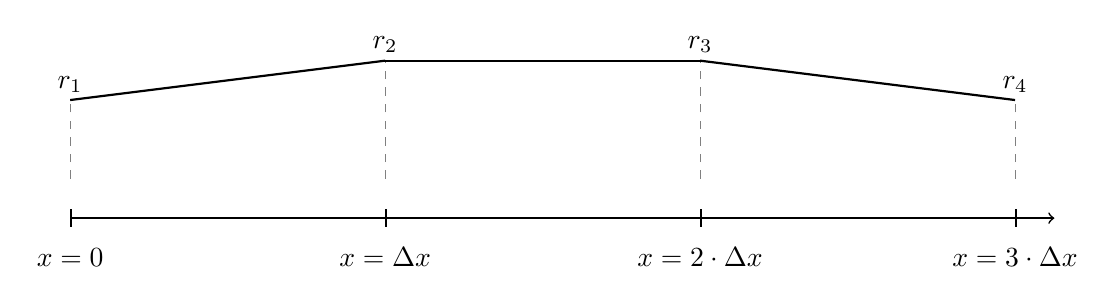
\begin{tikzpicture}
        \draw[dashed,color=gray] (0,0) -- (0,1);
        \draw[dashed,color=gray] (4,0) -- (4,1.5);
        \draw[dashed,color=gray] (8,0) -- (8,1.5);
        \draw[dashed,color=gray] (12,0) -- (12,1);
        \draw[thick] (0,1) -- (4,1.5);
        \draw[thick] (4,1.5) -- (8,1.5);
        \draw[thick] (8,1.5) -- (12,1);

        \draw[|-,semithick] (0,-0.5) -- (4,-0.5);
        \draw[|-,semithick] (4,-0.5) -- (8,-0.5);
        \draw[|-,semithick] (8,-0.5) -- (12,-0.5);
        \draw[|->,semithick] (12,-0.5) -- (12.5,-0.5);

        \draw (0,-1) node {$x=0$};
        \draw (4,-1) node {$x=\Delta x$};
        \draw (8,-1) node {$x=2 \cdot \Delta x$};
        \draw (12,-1) node {$x=3 \cdot \Delta x$};

        \draw (0,1.2) node {$r_1$};
        \draw (4,1.7) node {$r_2$};
        \draw (8,1.7) node {$r_3$};
        \draw (12,1.2) node {$r_4$};
    \end{tikzpicture}
    \caption{Фигура, путём вращения которой получаются усечённые конусы, составляющие мышцу.}
    \label{cone_plane}
\end{figure}

Для упрощения работы с моделью расстояние между узлами было выбрано постоянным. Данный факт не вносит никаких ограничений в представление модели, так как, описывая некоторый узел пропорционально соседям этого узла, получается представление, в котором визуально расстояние между этими двумя соседними узлами будет удвоено. Сделав обратное действие можно вводить новые узлы, уменьшая при этом расстояние между всеми узлами и увеличивая тем самым точность.

Учитывая описанное выше, для исчерпывающего описания состояния и положения мыщцы требуется, во-первых, массив радиусов оснований конусов в узлах, а во-вторых, расстояние между узлами.

Однако для исчерпывающего описания свойств мыщцы этого мало. Такой набор не хранит информации о поведении узлов при деформациях, поэтому также для каждого узла требуется добавить коэффициент приращения, который будет означать относительный прирост данного узла.
\begin{itemize}
    \item массив радиусов узлов;
    \item расстояние между узлами;
    \item массив коэффициентов прироста радиусов узлов.
\end{itemize}

\subsection{Расчёт формул деформации мышцы}

Как уже было сказано выше, общий объем модели составляется из объемов составляющих ее усечённых конусов, объем которых вычисляется как фигура вращения отрезка. 

Отрезок в данном случае проще всего задавать в виде прямой, заданной уравнением $ y = ax + b $, которая ограничена по \textit{x}: $x \in [0; \Delta x]$, где $\Delta x$ - расстояние между узлами. Рассматривать для $i$-ого и $(i + 1)$-ого узлов отрезок $[0; \Delta x]$ гораздо проще, чем отрезок $[(i - 1) \cdot \Delta x; i \cdot \Delta x]$, в связи с чем во всех последующих вычислениях подразумевается, что пара соседних узлов с индексами $i$ и $(i + 1)$ сдвигается на $(i - 1) \cdot \Delta x$ влево (можно заметить, что во всех последующих расчетах нас будет интересовать исключительно величина $\Delta x$, поэтому все последующие расчёты справделивы и для исходного положения составных частей модели). Площадь усечённого конуса в таком случае можно рассчитывать по формуле (\ref{for:area_rotate}):
\begin{equation}
    \label{for:area_rotate}
    \mathcal{V} = \pi \cdot \int_{0}^{\Delta x}f^2(x)dx,\qquad \text{где }f(x) = ax + b
\end{equation}

Далее можно подставить значение функции и рассчитать интеграл (\ref{for:area_opened}):
\begin{equation}
    \label{for:area_opened}
    \mathcal{V} = \pi \cdot \int_{0}^{\Delta x}\left(a^2x^2 + 2abx + b^2\right)dx = \pi \cdot \left(\frac{a^2x^3}{3} + abx^2 + b^2x\right)\Biggr|_{0}^{\Delta x}
\end{equation}

Из чего следует (\ref{for:open_limits}):
\begin{equation}
    \label{for:open_limits}
    \mathcal{V} = \pi \cdot \left(\frac{a^2\Delta x^3}{3} + ab\Delta x^2 + b^2\Delta x\right)
\end{equation}

Коэффициенты $a$ (угла наклона прямой) и $b$ (точки пересечения прямой с $Oy$) можно найти исходя из двух имеющихся точек отрезка. Так, для отрезка между $i$-ым и $(i+1)$-ым узлами, получается (\ref{for:coeffa}) и (\ref{for:coeffb}):
\begin{equation}
    \label{for:coeffa}
    a = \frac{y_{i+1} - y_{i}}{\Delta x}
\end{equation}

\begin{equation}
    \label{for:coeffb}
    b = y_i
\end{equation}

Пусть $n$ - кол-во узлов. Тогда $R = \{ r_1, r_2, \ldots r_n \}$ - массив радиусов узлов, $M = \{ m_1, m_2, \ldots, m_n \}$ - массив коэффициентов прироста радиусов узлов. Отсюда (учитывая формулы (\ref{for:open_limits}), (\ref{for:coeffa}) и (\ref{for:coeffb})) получается, что общий объем, для удобства последующих вычислений поделённый на $\pi$, можно вычислить по формуле (\ref{for:total_volume}):
\begin{equation}
    \label{for:total_volume}
    V = \frac{\mathcal{V}}{\pi} = \sum_{i=1}^{n-1} \left(\frac{(r_{i + 1} - r_i)^2 \cdot \Delta x}{3} + 2 r_i (r_{i + 1} - r_i) \cdot \Delta x + r_i^2 \Delta x \right)
\end{equation}

После выноса за знак суммы $\Delta x$ получается итоговая формула вычисления объема (\ref{for:total_volume_no_x}):

\begin{equation}
    \label{for:total_volume_no_x}
    V = \Delta x \cdot \sum_{i=1}^{n-1} \left(\frac{(r_{i + 1} - r_i)^2}{3} + 2 r_i (r_{i + 1} - r_1) + r_i^2 \right)
\end{equation}

Которую можно представить как функцию от расстояния между узлами $\Delta x$ и массива радиусов узлов (\ref{for:v_from_rads_dx}):
\begin{equation}
    \label{for:v_from_rads_dx}
    V(\Delta x, R) = \Delta x \cdot F(R), 
\end{equation}

где $F(R)$ - функция (\ref{for:f_r}):

\begin{equation}
    \label{for:f_r}
    F(R) = \sum_{i=1}^{n-1} \left(\frac{(r_{i + 1} - r_i)^2}{3} + 2 r_i (r_{i + 1} - r_1) + r_i^2 \right)
\end{equation}


Длина модели $L$ является суммой расстояний между узлами и для $n$ узлов находится следующим образом (\ref{for:len}):
\begin{equation}
    \label{for:len}
    L = (n - 1) \cdot \Delta x
\end{equation}

Откуда можно вывести зависимость расстояния между узлами от длины (\ref{for:del_from_len}):
\begin{equation}
    \label{for:del_from_len}
    \Delta x = \frac{L}{n - 1}
\end{equation}

При деформации модели (сокращении или растяжении) объем должен оставаться постоянным. Если посмотреть на выражение (\ref{for:v_from_rads_dx}) становится очевидным, что для равенства $V = V'$, где $V$ - объем до деформации, а $V'$ - после, должно выполнятся равенство (\ref{for:alter_eq}):
\begin{equation}
    \label{for:alter_eq}
    \Delta x \cdot F(R) = \Delta x' \cdot F(R')
\end{equation}

где $R'$ - массив радиусов узлов после деформации, $\Delta x'$, учитывая (\ref{for:del_from_len}), находится из (\ref{for:new_delta}):
\begin{equation}
    \label{for:new_delta}
    \Delta x' = \frac{L'}{n - 1} = \frac{L + \delta x}{n - 1} = \Delta x + \frac{\delta x}{n - 1}
\end{equation}

где $\delta x$ - изменение длины, а $L' = L + \delta x$ - новое значение длины модели.

Отсюда получается, что $F(R')$ можно найти, как (\ref{for:new_r}):
\begin{equation}
    \label{for:new_r}
    F(R') = \frac{F(R) \cdot \Delta x}{\Delta x'} = \frac{\Delta x}{\Delta x'} \cdot F(R)
\end{equation}

Пусть $\delta y$ - элементарное приращение радиуса. Тогда новое значение для радиуса каждого узла можно найти из соотношения:
\begin{equation}
    \label{for:new_rad}
    r_i' = r_i + m_i \cdot \delta y
\end{equation}
где $m_i$ (как было описано выше) - коэффициент прироста радиуса.

Таким образом можно выразить через (\ref{for:new_rad}) радиусы массива $R'$ и найти $F(R')$ как (\ref{for:f_r_new}):
\begin{equation}
    \label{for:f_r_new}
    \begin{split}
        F(R') = \sum_{i=1}^{n-1} (\frac{((r_{i + 1} + m_{i + 1} \cdot \delta y) - (r_i + m_{i} \cdot \delta y))^2}{3} + \\
        + 2 (r_i + m_i \cdot \delta y) \cdot (r_{i + 1} + m_{i + 1} \cdot \delta y - r_i + m{i} \cdot \delta y) + (r_i + m_i \cdot \delta y)^2)
    \end{split}
\end{equation}

После приведения подобных слагаемых относительно $\delta y$ получается (\ref{for:f_r_final}):
\begin{equation}
    \label{for:f_r_final}
        F(R') = A \delta y^2 + B \delta y + C,
\end{equation}

где $A$, $B$, $C$ рассчитываются из (\ref{for:coeffA}), (\ref{for:coeffB}), (\ref{for:coeffC}) соответственно.

\begin{equation}
    \label{for:coeffA}
    A = \sum_{i=1}^{n-1}\left(\frac{1}{3}m_{i + 1}^2 - \frac{5}{3}m_{i + 1}m_i + \frac{7}{3}m_i^2 \right)
\end{equation}

\begin{equation}
    \label{for:coeffB}
    B = \sum_{i=1}^{n-1}\left(m_{i + 1}r_i + m_ir_{i + 1} \right)
\end{equation}

\begin{equation}
    \label{for:coeffC}
    C = \sum_{i=1}^{n-1}\left(\frac{(r_{i + 1} - r_i)^2}{3} + r_{n + 1}r_n\right)
\end{equation}

Квадратное уравнение (\ref{for:f_r_final}) будет иметь решения (\ref{for:quad_sol}):
\begin{equation}
    \label{for:quad_sol}
    \delta y_{1, 2} = \frac{-B \pm \sqrt{B^2 - 4AC}}{2A}
\end{equation}

Среди решений больший интерес представляет большее, потому что меньшее решение находит сохранение объема при отрицательных радиусах, что не является верных в рамках имеющейся задачи. Таким образом $\delta y$ - больший корень среди корней из (\ref{for:quad_sol}), который равен (\ref{for:quad_sol_one}):
\begin{equation}
    \label{for:quad_sol_one}
    \delta y = \frac{-B + \sqrt{B^2 - 4AC}}{2A}
\end{equation}

Таким образом при деформации модели на величину $\delta x$ новые значения радиусов узлов будут иметь вид (\ref{for:new_rad}), где величина $\delta y$ находится из выражения (\ref{for:quad_sol_one}).

\subsection{Модель каркаса мышцы}

Каркас - модель, симулирующая в данной работе скелет руки 2 соединёнными концами стержнями, к которым крепится мышца. Каркас служит для улучшения визуализации мышцы и повышения реалистичности изображения. Положение каркаса может быть однозначно определено положением и состоянием модели мышцы, однако есть параметры, которые от нее не зависят - точки крепления. Для представления каркаса будет достаточно следующих параметров:
\begin{itemize}
    \item расстояние от нескрепленного конца первого стержня до точки крепления мышцы;
    \item расстояние от точки крепления мышцы к первому стержню до точки соединения стержней;
    \item расстояние от точки соединения стержней до точки крепления мышцы ко второму стержню;
    \item расстояние от точки крепления мышцы ко второму стержню до нескрепленного конца второго стержня;
\end{itemize}

Углы наклона стержней каркаса будут находится из теоремы косинусов, которая для треугольника с длинами сторон $A$, $B$, $C$ и угла $\alpha$, лежащего напротив стороны с длиной $A$, будет иметь вид (\ref{for:cos_th}):
\begin{equation}
    \label{for:cos_th}
    A^2 = B^2 + C^2 - 2BC \cos(\alpha)
\end{equation}

Откуда можно выразить угол $\alpha$ как (\ref{for:angle_from_th}):
\begin{equation}
    \label{for:angle_from_th}
    \alpha = \arccos{\left(\frac{B^2 + C^2 - A^2}{2BC}\right)}
\end{equation}

\section{Анализ алгоритмов удаления невидимых линий и поверхностей}

При выборе алгоритма удаления невидимых линий и поверхностей нужно учесть особенность поставленной задачи - работа программы будет выполняться в реальном режиме при взаимодействии с пользователем. Этот факт предъявляет к алгоритму требование по скорости работы. Для выбора наиболее подходящего алгоритма следует рассмотреть уже имеющиеся алгоритмы удаления невидимых линий и поверхностей.

\subsection{Алгоритм обратной трассировки лучей}
Алгоритм работает в пространстве изображения.

Идея: для определения цвета пиксела экрана через него из точки наблюдения проводится луч, ищется пересечение первым пересекаемым объектом сцены и определяется освещенность точки пересечения. Эта освещенность складывается из отраженной и преломленной энергий, полученных от источников света, а также отраженной и преломленной энергий, идущих от других объектов сцены. После определения освещенности найденной точки учитывается ослабление света при прохождении через прозрачный материал и в результате получается цвет точки экрана.

Плюсы:
\begin{itemize}
    \item качественное изображение, которое может быть построено с учётом явлений дисперсии лучей, преломления, а также внутреннего отражения;
    \item возможность использования в параллельных вычислительных системах.
\end{itemize}

Минусы:
\begin{itemize}
    \item трудоёмкие вычисления;
    \item высокая сложность реализации версии, учитывающей все физические явления.
\end{itemize}

\textbf{Вывод:} так как в поставленной задаче в первую очередь стоит требование быстроты работы алгоритма, а также ввиду того, что модели, использующиеся в программе, не являются прозрачными и имеют преимущественно диффузное отражение, данный алгоритм не подходит в рамках данной работы.

\subsection{Алгоритм, использующий Z-буфер}
Алгоритм работает в простанстве изображения.

Идея: имеется 2 буфера - буфер кадра, который используется для запоминания цвета каждого пиксела изображения, а также $z$-буфер - отдельный буфер глубины, используемый для запоминания координаты $z$ (глубины) каждого видимого пиксела изображения. В процессе работы глубина или значение $z$ каждого нового пиксела, который нужно занести в буфер кадра, сравнивается с глубиной того пиксела, который уже занесен в $z$-буфер. Если это сравнение показывает, что новый пиксел расположен выше пиксела, находящегося в буфере кадра ($z > 0$), то новый пиксел заносится в цвет рассматриваемого пиксела заносится в буфер кадра, а координата $z$ - в $z$-буфер. По сути, алгоритм является поиском по $x$ и $y$ наибольшего значения функции $z(x, y)$.

Плюсы:
\begin{itemize}
    \item возможность обработки поверхностей любой сложности;
    \item отсутствие требования сортировки объектов по глубине;
    \item высокая скорость работы.
\end{itemize}

Минусы:
\begin{itemize}
    \item требование большого объема памяти (в рамках современных вычислительных систем несущественно);
    \item сложность работы с прозрачными и просвечивающими объектами.
\end{itemize}

\textbf{Вывод:} ввиду того, что алгоритм удовлетворяет главному требованию программы, а его минусы не входят в число требований к программе, данный алгоритм может быть выбран в качестве алгоритма удаления невидимых линий и поверхностей в данной работе.

\subsection{Алгоритм Робертса}
Алгоритм работает в объектном пространстве. 

Идея: алгоритм прежде всего удаляет из каждого тела те ребра или грани, которые экранируются самим телом. Затем каждое из видимых ребер каждого тела сравнивается с каждым из оставшихся тел для определения того, какая его часть или части, если таковые есть, экранируются этими телами. 

Плюсы:
\begin{itemize}
    \item простые, но при этом точные математические методы;
    \item реализации алгоритма, использующие предварительную приоритетную сортировку вдоль оси z и простые габаритные или минимаксные тесты, демонстрируют почти линейную зависимость от числа объектов.
\end{itemize}

Минусы:
\begin{itemize}
    \item вычислительная трудоёмкость алгоритма теоретически растет, как квадрат числа объектов;
    \item большое количество этапов обработки и предварительных вычислений (из чего следует большое количество кода и высокая асимптотическая константа);
    \item отсутствие возможности работы с прозрачными и просвечивающими объектами.
\end{itemize}

\textbf{Вывод:} данный алгоритм сложен в реализации в виду большого количества требуемых оптимизаций, а так же будет работать медленнее с аппроксимированными фигурами вращения, нежели со стандартными многогранниками, что приведет к медленной работе и не будет удовлетворять главному требованию программы.

\subsection*{Вывод}

В таблице \ref{tab:cmp_del} представлено сравнение алгоритмов удаления невидимых линий и поверхностей (по каждому параметру составлен рейтинг: 1 - лучший алгоритм, 3 - худший). Так как главным требованием к алгоритму является скорость работы, алгоритмы были оценены по следующим критериям:
\begin{itemize}
    \item скорость работы (С);
    \item масштабируемость с ростом количества моделей (ММ);
    \item масштабируемость с увеличением размера экрана (МЭ);
    \item работа с объектами сложной формы (СФ).
\end{itemize}

\begin{table}[!h]
    \begin{center}
        \begin{tabular}{| @{\hspace{7mm}}r@{\hspace{7mm}} | @{\hspace{7mm}}r@{\hspace{7mm}} | @{\hspace{7mm}}l@{\hspace{7mm}} | @{\hspace{7mm}}l@{\hspace{7mm}} | @{\hspace{7mm}}l@{\hspace{7mm}} |}
        \hline
        Алгоритм & С & ММ & МЭ & СФ \\ 
        \hline
        Z-буфера & 1 & 2 & 1 & 1 \\
        Трассировка лучей & 3 & 1 & 3 & 2\\
        Робертса & 2 & 3 & 1 & 3\\ 
        \hline
        \end{tabular}
    \end{center}
    \caption{\label{tab:cmp_del} Сравнение алгоритмов удаления невидимых линий и поверхностей.}
\end{table}

С учётом результатов в таблице \ref{tab:cmp_del} был выбран алгоритм \textbf{Z-буфера} удаления невидимых линий и поверхностей.


\section{Анализ методов закрашивания}

Методы закрашивания используются для затенения полигонов (или поверхностей, аппроксимированных полигонами) в условиях некоторой сцены, имеющей источники освещения. С учётом взаимного положения рассматриваемого полигона и источника света находится уровень освещенности по закону Ламберта (\ref{for:lambert}):
\begin{equation}
    \label{for:lambert}
    I_{\alpha} = I_0 \cdot \cos{(\alpha)}
\end{equation}

где $I_{\alpha}$ - уровень освёщенности в рассматриваемой точке, $I_0$ - максимальный уровень освёщенности, а $\alpha$ - угол между вектором нормали к плоскости и вектором, направленным от рассматриваемой точки к источнику освещения (в случае нормированных векторов может быть рассчитан как скалярное произведение данных векторов).

\subsection{Простая закраска}

Идея: вся грань закрашивается одним уровнем интенсивности, который зависит высчитывается по закону Ламберта. При данной закраске все плоскости (в том числе и те, что аппроксимируют фигуры вращения), будут закрашены однотонно, что в случае с фигурами вращения будет давать ложные ребра.

Плюсы:
\begin{itemize}
    \item быстрая работа;
    \item хорошо подходит для многогранников, обладающих преимущественно диффузным отражением.
\end{itemize}

Минусы:

\begin{itemize}
    \item плохо подходит для фигур вращения: видны ребра.
\end{itemize}

\textbf{Вывод:} учитывая, что в рамках данной работы все модели - фигуры вращения, данных алгоритм не является подходящим.

\subsection{Закраска по Гуро}
Идея: билинейная интерполяция в каждой точке интенсивности освещения в вершинах.

Нормаль к вершине можно найти несколькими способами:
\begin{itemize}
    \item интерполировать нормали прилегающих к вершине граней;
    \item использовать геометрические свойства фигуры (так, например, в случае со сферой ненормированный вектор нормали будет в точности соответствовать вектору от центра сферы до рассматриваемой точки).
\end{itemize}

После нахождения нормали ко всем вершинам находится интенсивность в каждой вершине по закону Ламберта (\ref{for:lambert}).
Затем алгоритм проходится сканирующими строками по рассматриваемому полигону для всех $y: y \in [y_{min}; y_{max}]$. Каждая сканирующая строка пересекает 2 ребра многоугольника, пусть для определённости это будут ребра через одноименные вершины: $MN$ и $KL$. В точках пересечения высчитывается интенсивность путём интерполяции интенсивности в вершинах. Так, для точки пересечения с ребром $MN$ интенсивность будет рассчитана как (\ref{for:int_mn}):
\begin{equation}
    \label{for:int_mn}
    I_{MN} = \frac{l_1}{l_0} \cdot I_M + \frac{l_2}{l_0} \cdot I_N
\end{equation}
где $l_1$ - расстояние от точки пересечения до вершины $N$, $l_2$ - расстояние от точки пересечения до вершины $M$, $l_0$ - длина ребра $MN$.
Для точки пересечения сканирующей строки с ребром $KL$ интенсивность высчитывается аналогично.

Далее, после нахождения точек пересечения, алгоритм двигается по $Ox$ от левой точки пересечения $X_{left}$ до правой точки пересечения $X_{right}$ и в каждой точке $\mathcal{X}$ интенсивность рассчитывается как (\ref{for:int_x}):
\begin{equation}
    \label{for:int_x}
    I_{\mathcal{X}} = \frac{\mathcal{X} - X_{left}}{X_{right} - X_{left}} \cdot I_{X_{right}} + \frac{X_{right} - \mathcal{X}}{X_{right} - X_{left}} \cdot I_{X_{left}}
\end{equation}

Плюсы:
\begin{itemize}
    \item хорошо подходит для фигур вращения, аппроксимированных полигонами, с диффузным отражением.
\end{itemize}

Минусы:
\begin{itemize}
    \item при закраске многогранников ребра могут стать незаметными.
\end{itemize}

\textbf{Вывод:} с учетом наличия в данной работе исключительно фигур вращения данных алгоритм подходит гораздо больше предыдущего.


\subsection{Закраска по Фонгу}
Идея: данный алгоритм работает похожим на алгоритм Гуро образом, однако ключевым отличием является то, что интерполируются не интенсивности в вершинах, а нормали. Таким образом, закон Ламберта в данном алгоритме применяется в каждой точке, а не только в вершинах, что делает этот алгоритм гораздо более трудоёмким, однако с его помощью можно гораздо лучше изображаются блики.

Плюсы:
\begin{itemize}
    \item хорошо отображает блики, вследствие чего подходит для закраски фигур с зеркальным отражением.
\end{itemize}

Минусы:
\begin{itemize}
    \item самый трудоёмкий алгоритм из рассмотренных.
\end{itemize}

\subsection*{Вывод}

В таблице \ref{tab:cmp_paint} представлено сравнение алгоритмов закраски (по каждому параметру составлен рейтинг: 1 - лучший алгоритм, 3 - худший). Так как требованиями к алгоритму являются высокая скорость работы, а также возможность закраски фигур вращения с диффузными свойствами отражения, алгоритмы были оценены по следующим критериям:
\begin{itemize}
    \item скорость работы (С);
    \item работа с фигурами вращения (ФВ);
    \item работа с фигурами со свойствами диффузного отражения (ДО).
\end{itemize}

\begin{table}[!h]
    \begin{center}
        \begin{tabular}{| @{\hspace{7mm}}r@{\hspace{7mm}} | @{\hspace{7mm}}r@{\hspace{7mm}} | @{\hspace{7mm}}l@{\hspace{7mm}} | @{\hspace{7mm}}l@{\hspace{7mm}} |}
        \hline
        Алгоритм & С & ФВ & ДО \\ 
        \hline
        Простой & 1 & 3 & 1 \\
        Гуро & 2 & 1 & 1 \\
        Фонга & 3 & 1 & 3 \\ 
        \hline
        \end{tabular}
    \end{center}
    \caption{\label{tab:cmp_paint} Сравнение алгоритмов закраски.}
\end{table}

С учётом результатов в таблице \ref{tab:cmp_paint} был выбран алгоритм закраски \textbf{Гуро}.


\section*{Вывод}

В данном разделе были формально описаны модели мышцы, каркаса и законы, по которым эти модели деформируются, были рассмотрены алгоритмы удаления невидимых линий и поверхностей, методы закрашивания поверхностей. В качестве алгоритма удаления невидимых линий и поверхностей был выбран алгоритм z-буфера, в качестве метода закрашивания был выбран алгоритм закраски Гуро.
